\section{L’Analyse des liens}
\begin{itemize}
\item Concentrateurs ( Hubs )
\item Autorités ( Authorities )
\item Comment trouver la meilleure page ?
\end{itemize}

Voir figure ci-dessous \\	

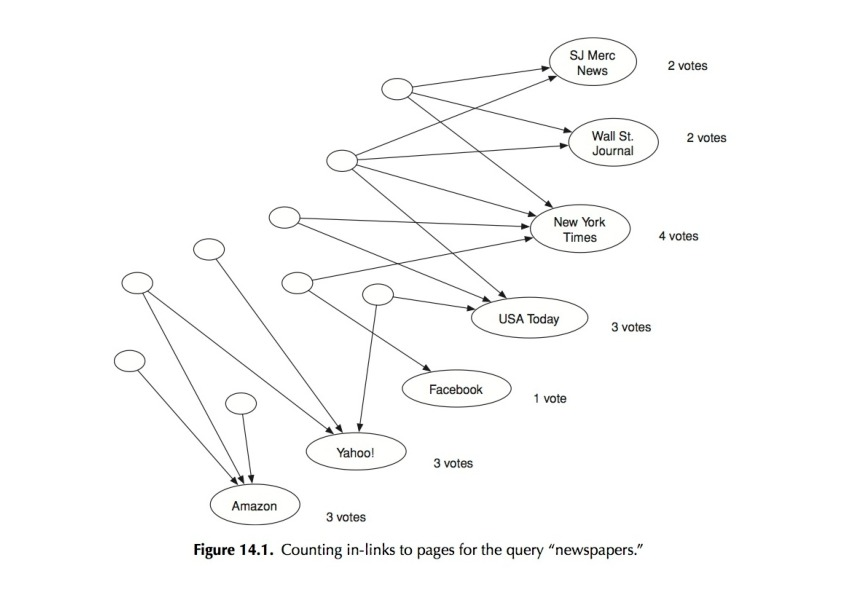
\includegraphics[scale=0.5]{images/ref/fig-14-1.jpeg}
\subsection{Requête News Papers}

\paragraph{Pourquoi Facebook, Yahoo, Amazon, se retrouvent-ils dans la requette News Papers ?}
Car beaucoup d'utilisateurs ont des pages concentrés sur ces sites et comme dans cet exemple on utilise un algorithme qui n'est pas très sophistiqué, elles apparaissent. 

\paragraph{Comment pouvoir trouver la meilleure page?}
\begin{enumerate}
\item Liens entrants $ \rightarrow $ votes
\item  Liens sortants  calcul du$ \rightarrow$  poids
\item Mise à jour des liens entrants
\item Mise à jour des liens sortants 
\end{enumerate}

\subsubsection{Algorithme}
Pages autorité (entrants (liens)) auto (p) \\
Pages concentrateurs (sortants ) conc (p)\\
Mises à jour :auto'(p) =  $ \sum_ {p'\rightarrow p}conc(p') $ \\
avec $p'\rightarrow p $ les pages p' qui ont un lien vers P  \\
conc'(p) = $ \sum_ {p\rightarrow p'}auto(p') $ \\
avec  $p \rightarrow p' $ les pages p' qui sont référencées à partir de p  \\

\subsubsection*{Itération}}

$ \forall p(page) $ : \[
\left \{
\begin{array}{r c l}
auto(p)  & = & 1 \\
conc (p)   & = & 1 \\

\end{array}
\right .
\]
 \\
 Mise à jour , normalisation, auto'(p) = $\frac{auto (p)}{  \sum auto(p')  }$\\
 conc' (p) = $\frac{conc (p)}{  \sum conc(p)  }$\\
 Cet algorithme converge \\
 \\
 En appliquant maintenant cet algorithme,  la Requête News Papers nous donnerait les résultats suivants:\\
 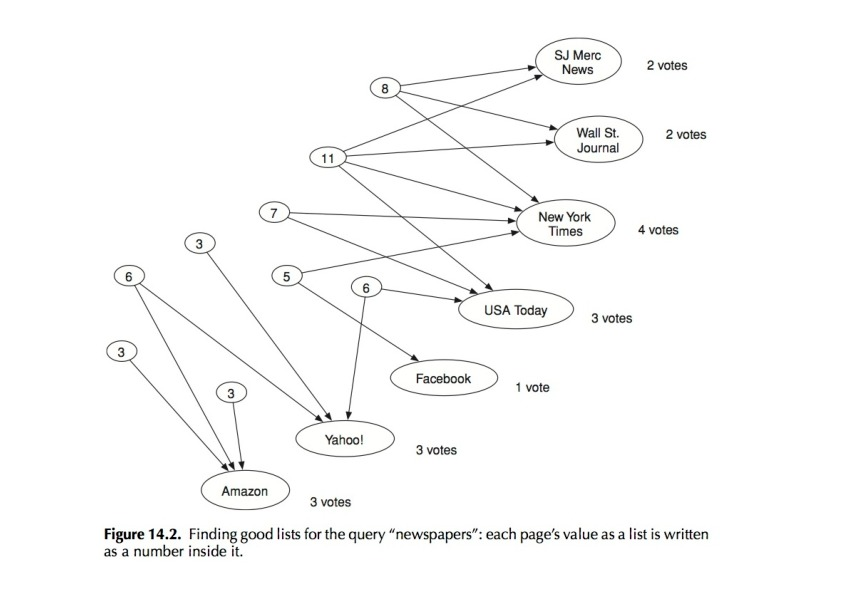
\includegraphics[scale=0.5]{images/ref/fig-14-2.jpeg}
 
 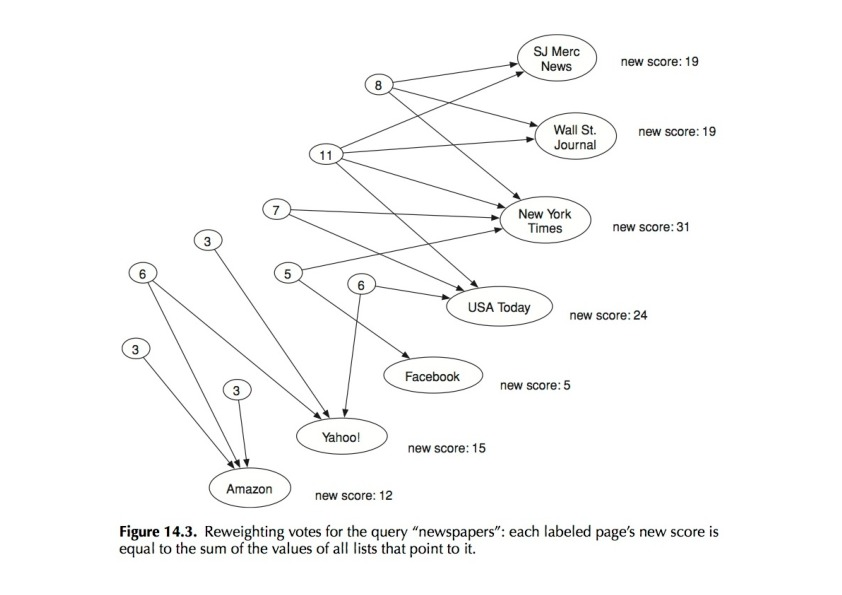
\includegraphics[scale=0.5]{images/ref/fig-14-3.jpeg}
 
 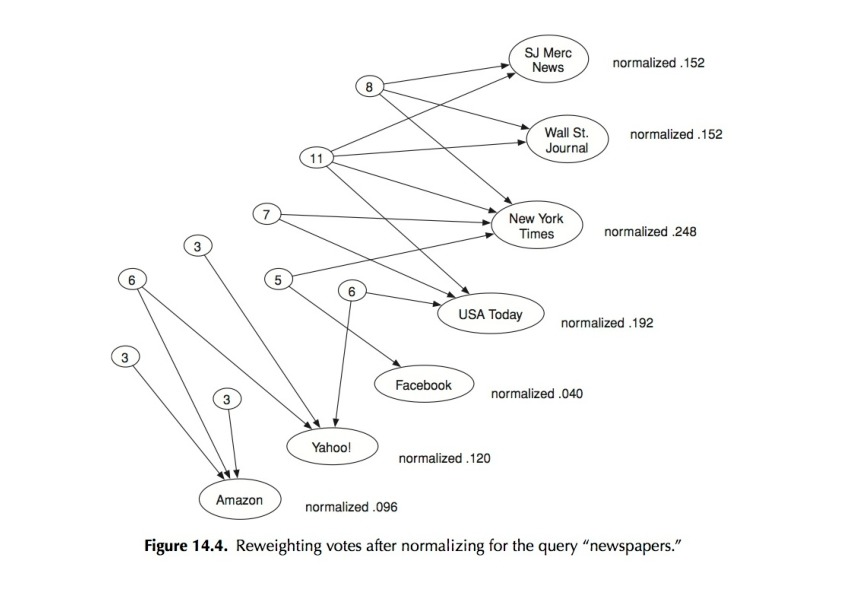
\includegraphics[scale=0.5]{images/ref/fig-14-4.jpeg}
 
 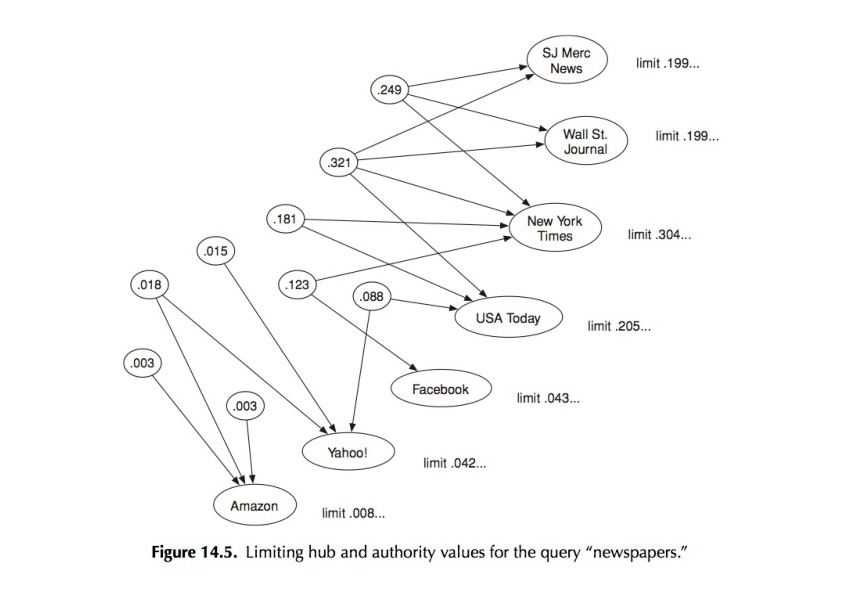
\includegraphics[scale=0.5]{images/ref/fig-14-5.jpeg}
	
 Comme nous pouvons voir, l'algorithme compte le nombre de liens entrants pour attribuer un poids à chaque place. Puis on normalise les valeurs trouvaient qui correspondent au poids de la page.
 Au plus grand est le poids d'une page au plus son autorité sera grande.\\
\section{PageRank}

- Consolider autorités et concentrateurs  \\
- Une valeur par noeud $ \rightarrow $ son "PageRank" que nous allons calculer. \\
- Intuition: Un "fluide" qui circule dans le réseau. \\
 \\
 \textbf{ Algorithme PageRank :}\\
 \\
 1) N noeuds (chaque noeud représentant une page) : Initialisation Pr(p) =  $\frac{1}{n}$\\
 2) Choisir un nombre de pas k\\
 3) K mises à jour:\\
 \\
 Pr(p) = $ \sum_ {p'}\frac{Pr(p')}{n(p')} $ avec n(p') le nombre de liens sortant de p' et Pr(p') le poids (ou PageRank de p') à la $k^{ème}$ itération.\\
 \\
 \textbf{Exemple de PageRank :}\\
 \\
 Voir graphe ci-dessous : \\
 
 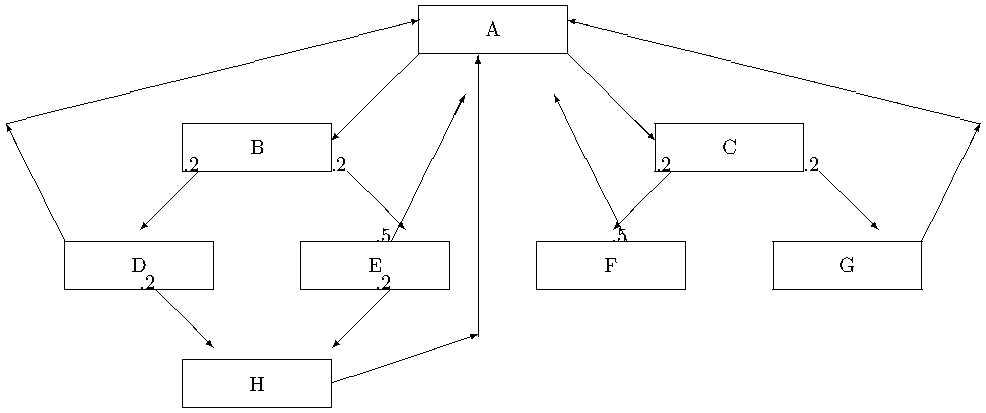
\includegraphics[scale=0.8]{images/24_imagePr.pdf}
 
 	\begin{tabular}{|c| c |c |c |}
		\hline
		Noeuds/Itérations & 0 & 1 & 2 \\
		\hline
		A & 1/8 & 1/2 & 5/16 \\
		B & 1/8 & 1/16 &  1/4   \\
		C & 1/8 & 1/16 & 1/4    \\
		D & 1/8 & 1/16 & 1/32  \\
		E & 1/8 & 1/16 &  1/32   \\
		F & 1/8 & 1/16 & 1/32    \\
		G & 1/8 & 1/16 & 1/32    \\
		H & 1/8 & 1/8 &  1/16   \\
		\hline
		$\sum $ & 1 & 1 & 1 \\
		\hline
	\end{tabular}

 Si nous continuons à laisser travailler l'algorithme, pour un nombre n fini d'itérations telles que k=n, il y aura convergence de l'algorithme. Dans cet exemple-ci,  nous aurons :\\
 \\
 Pr(A) = 4/13 ; Pr(B) = 2/13 ; Pr(C) = 2/13 ; Pr(Autres) = 1/13 \\
 Et la condition $ \sum Pr(p) = 1 $ est toujours vérifiée .
 
 L'équilibre est vérifié si le graphe est connexe, s’il ne l'est pas un problème se pose: Le fluide peut arriver au mauvais noeud (analogie réseau d'eau )  :

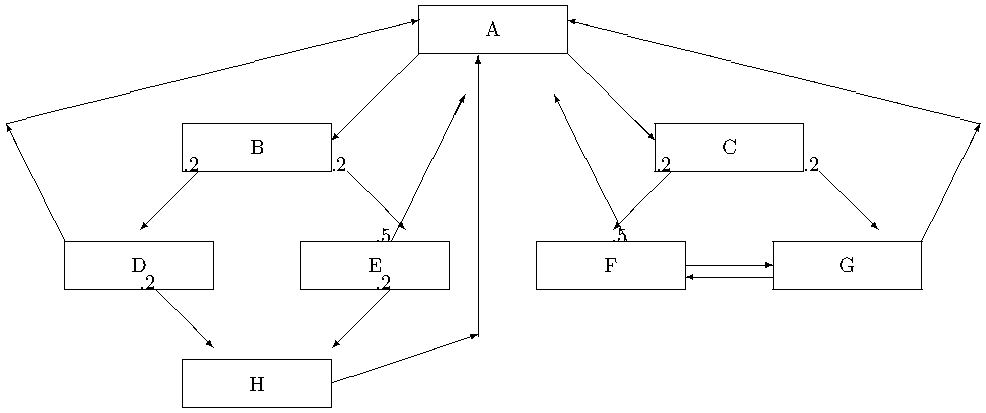
\includegraphics[scale=0.8]{images/24_Nconnexe.pdf}

\subsubsection*{Solution du problème}
\begin{itemize}
\item Fermer la boucle
\item Créer des cycles
\item Analogie : Circulation d'eau dans l'atmosphère
\end{itemize}
 	Il faut un peu de fluide partout dans chaque itération.\\
 	Nouvelle règle de mise à jour : \\
 	
      Pr(p) = $ \sum_ {p'}\frac{Pr(p')}{n(p')} $ (ancien) \\
     \\
         Pr(p) = Sx(Pr(p) + (1-S)x$\frac{1}{n}$) \\
         S est un paramètre : $ 0 \le S \le 1 $ \\
         \\
        \textbf{ Autre manière de voir l'algorithme :} \\
        \\
        Marche aléatoire : 
        \\
        Probabilité de S : Suivre un lien \\
        (1-S) : Choisi un nœud au hasard \\
        $\rightarrow $ La même valeur pour Pr(p) \\
        PageRank : (début 1990) \\
        - Abandon partiel en 2003/2004 à cause de SEO : Search engine optimisation (Tricheurs )
